In order to convert the constrained highway dimension to hub labels, we first convert the original graph $G$ into an \emph{augmented graph} $G^B$ under which the efficient paths are now shortest paths by enforcing the following properties
%For a fixed parameter $B\in \N$, we construct a structure that allows to obtain $\dist(s,d|b)$ for any $b\leq B$.
%Additionally, we will always answer with an efficient path, so there could be a ``surplus of budget''.
%On an intuitive level, we create a graph with the following properties:
\begin{enumerate}[nosep]
\item All paths starting from a given node are feasible, i.e., they satisfy the budget constraint.
\item Efficient paths become shortest paths.
\item The use of ``unnecessary resource'' is penalized, hence inefficient paths are not shortest.
\end{enumerate}

We give now the formal description of the augmented graph.
Consider nodes as pairs of the form $\pp{v,b}$. 
This encodes the information of remaining resource $b\geq 0$ and location $v\in V$.
A node is connected to neighbours (according to $E$) as long as the remaining resource of that transition is non-negative.
Finally, we create $n$ sink nodes, denoted $v^-$.


\begin{definition}
Given a network $(G,\ell)$ and $B\in\N$, the augmented version $G^B=(V^B,E^B)$ is defined by
\begin{align*}
V^B &:=\crl*{\pp{v,b}: v\in V, b=0,1,\ldots,B}\cup\crl*{v^-:v\in V},\\
E^B &:=\crl*{\pp{v,b}\pp{v',b'} : vv'\in E, b'=b-c_{vv'}, b'\geq 0}\cup E^{B}_{-},\\
E^{B}_{-} &:= \crl*{\pp{v,b}v^-: v\in V, B\geq b\geq 0}.
\end{align*}
The lengths to sink nodes are $\ell(\pp{v,b},v^-)=\frac{1}{b+1}$.
The other lengths are preserved, i.e., $\ell(\pp{v,b},\pp{v',b'})=\ell(vv')$.
\end{definition}

\begin{figure}\caption{Example of an augmented graph}\label{fig:augmented}
\begin{center}
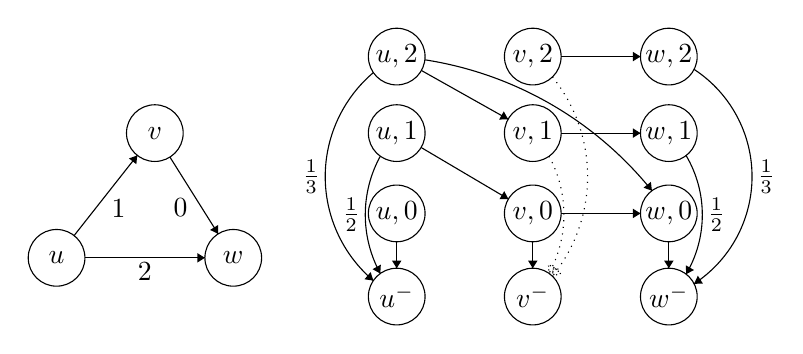
\begin{tikzpicture}[scale=0.12]
\tikzstyle{every node}+=[inner sep=0pt]
\draw [black] (5,-34.3) circle (3);
\draw (5,-34.3) node {$u$};
\draw [black] (15.4,-21.1) circle (3);
\draw (15.4,-21.1) node {$v$};
\draw [black] (23.7,-34.3) circle (3);
\draw (23.7,-34.3) node {$w$};
\draw [black] (41,-13) circle (3);
\draw (41,-13) node {$u,2$};
\draw [black] (41,-21.1) circle (3);
\draw (41,-21.1) node {$u,1$};
\draw [black] (41,-29.6) circle (3);
\draw (41,-29.6) node {$u,0$};
\draw [black] (41,-38.4) circle (3);
\draw (41,-38.4) node {$u^-$};
\draw [black] (55.4,-13) circle (3);
\draw (55.4,-13) node {$v,2$};
\draw [black] (55.4,-21.1) circle (3);
\draw (55.4,-21.1) node {$v,1$};
\draw [black] (55.4,-29.6) circle (3);
\draw (55.4,-29.6) node {$v,0$};
\draw [black] (55.4,-38.4) circle (3);
\draw (55.4,-38.4) node {$v^-$};
\draw [black] (69.8,-13) circle (3);
\draw (69.8,-13) node {$w,2$};
\draw [black] (69.8,-21.1) circle (3);
\draw (69.8,-21.1) node {$w,1$};
\draw [black] (69.8,-29.6) circle (3);
\draw (69.8,-29.6) node {$w,0$};
\draw [black] (69.8,-38.4) circle (3);
\draw (69.8,-38.4) node {$w^-$};
\draw [black] (6.86,-31.94) -- (13.54,-23.46);
\fill [black] (13.54,-23.46) -- (12.66,-23.78) -- (13.44,-24.39);
\draw (10.77,-29.12) node [right] {$1$};
\draw [black] (17,-23.64) -- (22.1,-31.76);
\fill [black] (22.1,-31.76) -- (22.1,-30.82) -- (21.25,-31.35);
\draw (18.92,-29) node [left] {$0$};
\draw [black] (8,-34.3) -- (20.7,-34.3);
\fill [black] (20.7,-34.3) -- (19.9,-33.8) -- (19.9,-34.8);
\draw (14.35,-34.8) node [below] {$2$};
\draw [black] (43.98,-13.342) arc (81.20715:38.87551:38.409);
\fill [black] (68.01,-27.19) -- (67.9,-26.26) -- (67.12,-26.88);
\draw [black] (43.58,-22.62) -- (52.82,-28.08);
\fill [black] (52.82,-28.08) -- (52.38,-27.24) -- (51.87,-28.1);
\draw [black] (58.4,-29.6) -- (66.8,-29.6);
\fill [black] (66.8,-29.6) -- (66,-29.1) -- (66,-30.1);
\draw [black] (43.61,-14.47) -- (52.79,-19.63);
\fill [black] (52.79,-19.63) -- (52.33,-18.8) -- (51.84,-19.67);
\draw [black] (58.4,-21.1) -- (66.8,-21.1);
\fill [black] (66.8,-21.1) -- (66,-20.6) -- (66,-21.6);
\draw [black] (58.4,-13) -- (66.8,-13);
\fill [black] (66.8,-13) -- (66,-12.5) -- (66,-13.5);
\draw [black] (72.471,-14.353) arc (56.79859:-56.79859:13.561);
\fill [black] (72.47,-37.05) -- (73.41,-37.03) -- (72.87,-36.19);
\draw (79.11,-25.7) node [right] {$\frac{1}{3}$};
\draw [black] (71.625,-23.471) arc (30.61438:-30.61438:12.329);
\fill [black] (71.63,-36.03) -- (72.46,-35.59) -- (71.6,-35.09);
\draw (73.84,-29.75) node [right] {$\frac{1}{2}$};
\draw [black] (69.8,-32.6) -- (69.8,-35.4);
\fill [black] (69.8,-35.4) -- (70.3,-34.6) -- (69.3,-34.6);
\draw [black] (38.528,-36.71) arc (-130.31667:-229.68333:14.439);
\fill [black] (38.53,-36.71) -- (38.24,-35.81) -- (37.59,-36.57);
\draw (32.93,-25.7) node [left] {$\frac{1}{3}$};
\draw [black] (39.265,-35.961) arc (-151.22419:-208.77581:12.903);
\fill [black] (39.26,-35.96) -- (39.32,-35.02) -- (38.44,-35.5);
\draw (37.17,-29.75) node [left] {$\frac{1}{2}$};
\draw [black] (41,-32.6) -- (41,-35.4);
\fill [black] (41,-35.4) -- (41.5,-34.6) -- (40.5,-34.6);
\draw [black] (55.4,-32.6) -- (55.4,-35.4);
\fill [black] (55.4,-35.4) -- (55.9,-34.6) -- (54.9,-34.6);
\draw [dotted] (57.481,-15.155) arc (38.87983:-38.87983:16.799);
\draw [densely dotted] (57.48,-36.24) -- (58.37,-35.94) -- (57.59,-35.31) -- cycle;
\draw [dotted] (57.121,-23.549) arc (28.47781:-28.47781:13.004);
\draw [densely dotted] (57.12,-35.95) -- (57.94,-35.49) -- (57.06,-35.01) -- cycle;
\end{tikzpicture}
\end{center}
\end{figure}

An illustration of the construction is presented in Figure~\ref{fig:augmented}.
The original graph is on the left with labelled costs and unit lengths.
On the right is the augmented version, the unlabelled lengths are $1$.
We did not draw the links to the sinks $u^-,v^-$ for exposition purposes. 

\begin{remark}
The edge costs are allowed to be zero, therefore the augmented graph may contain cycles.
On the other hand, the dynamic programming approach requires a DAG \cite{alex_bicriteria}; the topological order is what ensures the efficiency of the algorithm.
\end{remark}

We map paths in $G^B$ to paths in $G$ in the intuitive way.
The augmented path is projected by removing the budget labels and sink nodes.
Formally,

\begin{definition}
Let $P$ be a path in $G^B$.
If $P$ is of the form $\pp{v_1,b_1}\ldots\pp{v_k,b_k}$, then the projection of $P$, denoted $\bar P$, is the path $\bar P\defeq v_1v_2\ldots v_k$.
Analogously, if $P$ is of the form $\pp{v_1,b_1}\ldots\pp{v_k,b_k}v_{k}^-$, then $\bar P:=v_1\ldots v_{k}$. 
\end{definition}


\begin{proposition}\label{prop:shorteffic}
A shortest path from $\pp{s,b}$ to a sink node $t^-$ projects to an efficient path in $G$ solving $\dist(s,t|b)$. 
\end{proposition}
\begin{proof}
Let $P$ be the shortest path from $\pp{s,b}$ to $t^-$.
To reach $t^-$, $P$ must pass trough some $\pp{t,b'}$, $b'\geq 0$.
By construction, $P$ consumes $b-b'$ units of resource, hence it is feasible.
Note that $\bar P$ is the shortest among $(s,t)$-paths with cost $b-b'$.

Assume, by way of contradiction, that $\bar P$ is not efficient.
As $\bar P$ is the shortest using $b-b'$ units of resource, there exists $P'$ such that $\ell(\bar P')\leq \ell(\bar P)$ and $c(\bar P')< c(\bar P)$.
It must be that $P'$ passes through $\pp{t,b''}$, with $b''>b'$.
We argue that, in this case, $P$ would not be a shortest path to $t^-$.
Indeed, 
\[
\ell(P')=\ell(\bar P')+\frac{1}{1+b''}
\leq \ell(\bar P) +\frac{1}{1+b''}
< \ell(\bar P) +\frac{1}{1+b'},
\]
where the last expression is exactly $\ell(P)$.
\end{proof}

Using the previous result, we can construct LSHS in the augmented graph using the EPHS of the original graph.
It is interesting that, assuming doubling dimension $\alpha$ and $\beta$-witness, we obtain sparsity of $\alpha^{\beta} hB$ and thus query times of $O(\alpha^{\beta} hB\log D)$ \anote{now the witness is defined later}.
This is much better than the $O(Bn\Delta)$ of dynamic programming, but it is still pseudo-polynomial.
We observe that the query time can be made strongly polynomial if and only if the Pareto frontier contains at most a poly-logarithmic number of points.
See Section~\ref{sec:frontier} for a further discussion on this.
 
In $G^B$ we are not interested in every shortest path, but only on those ending in sink nodes, since these are projected to efficient paths. 
Let $\calP^B$ be such system, i.e., all shortest paths in $G^B$ ending in a sink node.
A hitting set for $\PE$ can be used to obtain a hitting set for $\calP^B$, but, since we require more information by augmenting the graph, the sparsity increases.
 
\begin{proposition}
Assume the system $\PE$ admits $(\hc,r)$-EPHS.
Then, $\calP^B$ admits $(\hc B,r)$-LSHS.
\end{proposition}
\begin{proof}
We define a set $C^B$ and prove that hits $\calP_r^B$ and that it is locally sparse.
Call $C$ the $(\hc,r)$-EPHS for $\PE$.
Define
\begin{equation}\label{eq:hitset}
C^B:=\{\pp{v,b}: v\in C, v \text{ hits }\bar P\in\calP_r^B, c(\bar P)=b\leq B \}.
\end{equation}

By Proposition~\ref{prop:shorteffic}, we know that shortest paths are efficient, hence $C^B$ hits all the desired paths.
Finally, we prove local sparsity.
Take any node $\pp{u,b}$ and observe that
\begin{align*}
\Bf_{2r}(\pp{u,b}) &= \{\pp{v,x}: \exists P\in\calP_{u,v}, \ell(P)\leq 2r, c(P)=b-x\} \\
&\subseteq \{\pp{v,x}: v\in \Bf_{2r}(u), x\leq b\} .
\end{align*}
We know that $\card{\Bf_{2r}(u)\cap C}\leq \hc$, therefore $\card{\Bf_{2r}(\pp{u,b})\cap C^B}\leq\hc b\leq \hc B$.
A similar argument shows the sparsity for the backward ball.
\end{proof}

\begin{remark}
The proof shows a stronger result.
In Equation~(\ref{eq:hitset}) we see that the sparsity around the node $\pp{u,b}$ is $\hc b$.
This will be key for the query time guarantee.
\end{remark}

The last result shows how LSHS translate to the augmented graph.
Since the notion of HD is much stronger, it is not always possible to make the analogous between two path systems.
Surprisingly, in this case we are able to relate the HD of both path systems.

\begin{proposition}\label{prop:HDaugmented}
If the HD of the system $\PE$ is $h_c$, then the HD of the system $\calP^B$ is $Bh_c$.
\end{proposition}
\begin{proof}
Fix $r>0$ and $\pp{v,b}\in V^B$ .
Let $H_{v,r}\subseteq V$ be the set hitting $S_r(v,\PE)$ and define $H:=H_{v,r}\times\{0,1,\ldots,B\}$.
We show that $H$ hits $\Sf_r(\pp{v,b},\calP^B)$.

Take $P\in\Sf_r(\pp{v,b},\calP^B)$.
Since $\dist(\pp{v,b},P)\leq 2r$, it holds $\dist(v,\bar P)\leq 2r$, therefore $\bar P\in \Sf_r(v,\PE)$.
Finally, $H_{v,r}$ hits $\bar P$, thus $H$ hits $P$.
A similar argument shows that $H$ hits $\Sb_r(\pp{v,b},\calP^B)$.
\end{proof}
